
\documentclass[a4paper]{article}

%% Language and font encodings
\usepackage[T1,T8K,T8M]{fontenc}
\usepackage[utf8]{inputenc}
\usepackage[english,georgian]{babel}

%% Sets page size and margins
\usepackage[a4paper,top=3cm,bottom=2cm,left=3cm,right=3cm,marginparwidth=1.75cm]{geometry}

%% Useful packages
\usepackage{amsmath}
\usepackage{graphicx}
\usepackage[colorinlistoftodos]{todonotes}
\usepackage[colorlinks=true, allcolors=blue]{hyperref}
\usepackage{float}
\usepackage{enumerate}
\usepackage{subfig}

\title{კეპლერის კანონები}
\author{ლეევან კანკაძე}

\begin{document}
	\maketitle
	
	\begin{abstract}
		კეპლერის კანონები.
	\end{abstract}
	
	\section{სტატიკა} სტატიკაში შეისწავლება მყარი სხეულების წონასწორობა, რომელზეც მოქმედებს ძალები. წონასწორობაში იგულისხმება მდგომარეობა, რომლისთვისაც, სხეულს არ გააჩნია აჩქარება, ანუ მოძრაობს თანაბრად და წრფივად, ან ნაწილობრივ, იმყოფება უძრავად ათვლის ინერციულ სისტემაში. (პრაქტიკულად ამოცანებში, დედამიწასთან დაკავშირებული ათვლის სისტემა ითვლება ინერციულად.
	
	რა ძალები მოქმედებს წონასწორობაში მყოფ სხეულზე? პირველ რიგში უნდა გავიხსენოთ სიმძიმის ძალა. ეს სიმძიმის ძალა არის ტოლქმედი სხეულის შემადგენელი ნაწილაკების სიმძიმის ძალისა.
	\section{შენახვის კანონები}
	\textbf{01.} $m$ მასის უძრავ ბირთვს $V$ სიჩქარით ეჯახება $M$ მასის მოძრავი ბირთვი. იპოვეთ ბირთვების სიჩქარეები დაჯახების შემდეგ, თუ დაჯახება დრეკადია და ცენტრული. ძალის მოქმედებს წრფე გადის სხეულის მასათა ცენტრზე - სიმძიმის ცენტრი.
		
	\section{ჭოჭონაქები}
	\textbf{01.} იპოვეთ რა ძალით მოქმედებს ჭერზე, ნახატზე გამოსახული უმასო ჭოჭონაქების სისტემა. თოკები უჭიმვადია და უმასო,  თითოეული სხეულის მასაა $m$.  ხახუნი უგულებელყავით.
	 			\begin{figure}[H]
	 			\centering
           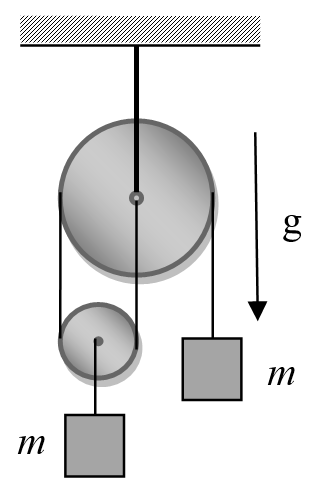
\includegraphics[width=0.2\columnwidth]{figures/03}
           \caption{A boat.}
           \label{fig:boat1}
        \end{figure}
	 
	\section{წრეწირზე მოძრაობა}
	 \textbf{01.} მოტოციკლეტისტი მოძრაობს ჰორიზონტალურ ზედაპირზე $v = 70$ კმ/სთ სიჩქარით, ბრუნდება $R = 100$ მ რადიუსის მოსახვევში, რა კუთხით უნდა გადაიხაროს რომ არ დაეცეს? \\
	 ამოხსნა\\
	 აქაც ხახუნის ძალაა, ძალა რომელცც აჩერებს მოტოცეკლისტს, $F_{fr} = \frac{m v^2}{R}$, საყრდენის რეაქციის ძალა $N = mg$. მომენტების წესი სიმძიმის ცენტრის მიმართ მომცემს განტოლებას $F_{fr}\cdot l \sin \alpha = N l \cos \alpha$. აქ მოცემული არაა $\mu$ და მაგიტომ გვჭირდება. ეს მომენტები.
	 
	\textbf{02.} რა მაქსიმალური $v$ სიჩქარით შეიძლება იმოძრავოს მანქანამ $\alpha$ კუთხით დახრილ სიბრტყეზე თუ სიმრუდის რადიუსია $R$ და ხახუნის კოეფიციენტი ბორბლებსა და გზას შორის არის $k$.
			\begin{figure}[H]
           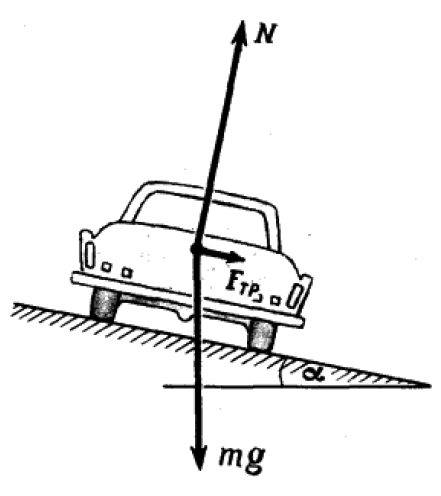
\includegraphics[width=0.2\columnwidth]{figures/02}
           \caption{A boat.}
           \label{fig:boat1}
        \end{figure}
	 
	\section{კეპლერის კანონები}
	\subsection{კეპლერის პირველი კანონი}
	პლანეტები მოძრაობს ელიფსებზე, რომელთა ერთ-ერთ ფოკუსში იმყოფება მზე.
	\subsection{კეპლერის მეორე კანონი}
	პლანეტის რადიუს-ვექტორი დროის ტოლ შუალედებში ტოლ ფართობებს მოხვეტს.
	\subsection{კეპლერის მესამე კანონი}
	პლანეტების გარშემოვლის პერიოდების კვადრატები ისე შეეფარდება ერთმანეთს, როგორც მათი ორბიტების დიდი ნახევარღერძების კუბები.
	\begin{equation}
		\frac{T_1^2}{T_2^2} = \frac{a_1^3}{a_2^3}
	\end{equation}
	\section{გრავიტაციული ურთიერთქმედების პოტენციალური ენერგია}
	$r$ მანძილით დაშორებული $m_1$ და $m_2$ მასის ნივთიერი წერტილების გრავიტაციული ურთიერთქმედების პოტენციალური ენერგიის ფორმულის მიღებას ინტეგრების ცოდნა სჭირდება. ჩვენ მოვიყვანთ შედეგს გამოყვანის გარეშე:
	\begin{equation}
		U = -G\frac{m_1 m_2}{r} + C
	\end{equation}
სადაც $C$ ნებისმიერი მუდმივაა. მისი კონკრეტული მნიშვნელობა დამოკიდებულია ნულოვანი დონის არჩევაზე. ჩვეულებრივ, ნულად თვლიან
უსასრულოდ დაშორებული სხეულების პოტენციალურ ენერგიას. ამ შემთხვევაში	$C = 0$ და $$U = -G\frac{m_1 m_2}{r}$$.
	
	\section{კოსმოსური სიჩქარეები}
	\subsection{პირველი კოსმოსური სიჩქარე}
		პირველი კოსმოსური სიჩქარე არის ის სიჩქარე, რომელიც საჭიროა სხეულს მივანიჭოთ გასროლისას რომ არ დაეცეს დედამიწაზე და გააგრძელოს მის გარშემო ბრუნვა. ნიუტონის მეორე კანონით:
		\begin{equation}
			\frac{mv^2}{r_E} = G\frac{M_Em}{r_E^2}
		\end{equation}
სადაც $M_E$ არის დედამიწის მასა, $r_E$ არის დედამიწის რადიუსი. რიცხვით გამოთვლისას მიიღება რომ $v = 7.91 \cdot 10^3$ მ/წმ.

	\subsection{მეორე კოსმოსური სიჩქარე}
		მეორე კოსმოსური სიჩქარის მინიჭებისას სხეულს შეუძლია დატოვოს დედამიწის ორბიტა, თუკი ჩავწერთ სრულ მექანიკურ ენერგიას. 
			\begin{equation}
				E = \frac{mv^2}{2} - G\frac{M_E m}{r_E}
			\end{equation}
ცხადოა როდესაც დედამიწის დატოვებს მას აღარ ექნება დედამიწასთან ურთიერთქმედების პოტენციალური ენერგია, და რადგან მინიმალურ სიჩქარეს ვეძებთ აღარც კინეტიკური ენერგია ექნება ორბიტის დატოვებისას მაშინ.
			\begin{equation}
				\frac{mv^2}{2} - G\frac{M_E m}{r_E} = 0
			\end{equation}
აქედან მივიღებთ:
			\begin{equation}
				v = \sqrt{\frac{2GM_E}{r_E}}
			\end{equation}
სადაც $M_E$ არის დედამიწის მასა, $r_E$ არის დედამიწის რადიუსი. რიცხვით გამოთვლისას მიიღება რომ $v = 11.2 \cdot 10^3$ მ/წმ.

ორივე შემთხვევაში შეიძლება გამოვიყენოთ მიახლოება, $g = GM/r_E^2$ და ზემო განტოლებებში ჩავსვათ.


\section{ამოცანები}
\textbf{01.} რა დროში დაეცემა მთვარე დედამიწას თუ ის სწრაფად გაჩერდება.\\
ამოხნსა: ამ ამოცანაში უნდა გამოვიყენოთ კეპლერის მესამე კანონი:
	\begin{equation}
		\frac{T_1^2}{T_2^2} = \frac{a_1^3}{a_2^3}
	\end{equation}
დავარდნა შეიძლება განვიხილოთ როგორც ძალიან გაწელილი ელიფსი. თუ დავუშვებთ რომ თავიდან მთვარის რადიუსი იყო $a$ ახალი რადიუსი იქნება $a/2$, მაშინ ვარდნის დრო იქნება.
	\begin{equation}
		T_1^2 = T_2^2\cdot\frac{(a/2)^3}{a^3} = T_2^2 \frac{1}{8}
	\end{equation}
სადაც $T_2$ არის ძველი მთვარის პერიოდი, მაშინ დავარდნის დრო იქნება პერიოდის ნახევარი $T_1/2$

\textbf{02.} უძრავად დამაგრებული $M$ მასის ნივთიერი წერტილის გრავიტაციულ ველში დიდი მანძილით დაშორებული წერტილიდან (ამ მანძილზე
გრავიტაციული ურთიერთქმედება შეგვიძლია უგულებელვყოთ) $v$ სიჩქარით მოძრაობს $m$ მასის ნივთიერი წერტილი, რომლის სამიზნე პარამეტრია $\rho$. იპოვეთ უმცირესი მანძილი ნივთიერ წერტილებს შორის.
		\begin{figure}[H]
           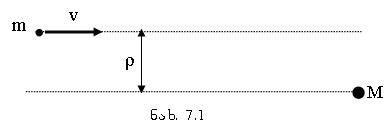
\includegraphics[width=0.2\columnwidth]{figures/fig_1}
           \caption{A boat.}
           \label{fig:boat1}
        \end{figure}
        
ამოხსნა:	იხსნება იმპულსის მუდმივობისა და ენერგიის მუდმივობით.\\
პასუხი: $$ r_{min} = \frac{1}{v^2} $$

\end{document}